% Round 3 agent architecture, one page. Build: xelatex architecture.tex
\documentclass[10pt]{article}
\usepackage[a4paper,landscape,margin=10mm]{geometry}
\usepackage{fontspec}
\setmainfont{Helvetica Neue}
\usepackage{tikz}
\usetikzlibrary{positioning,arrows.meta,calc}
\pagestyle{empty}
\setlength{\parindent}{0pt}
\begin{document}
\begin{center}
{\Large\bfseries Two-speed market agent — student 25620027, Round 3 on kit v4}\\[3pt]
{\small Seconds: a deterministic trade loop over the kit's real stock, driven by a policy table. Minutes: a model rewrites that table from the public ledger. Dashed boxes are kit v4, unchanged. Everything solid is this submission.}
\end{center}
\vspace{2mm}
\begin{center}
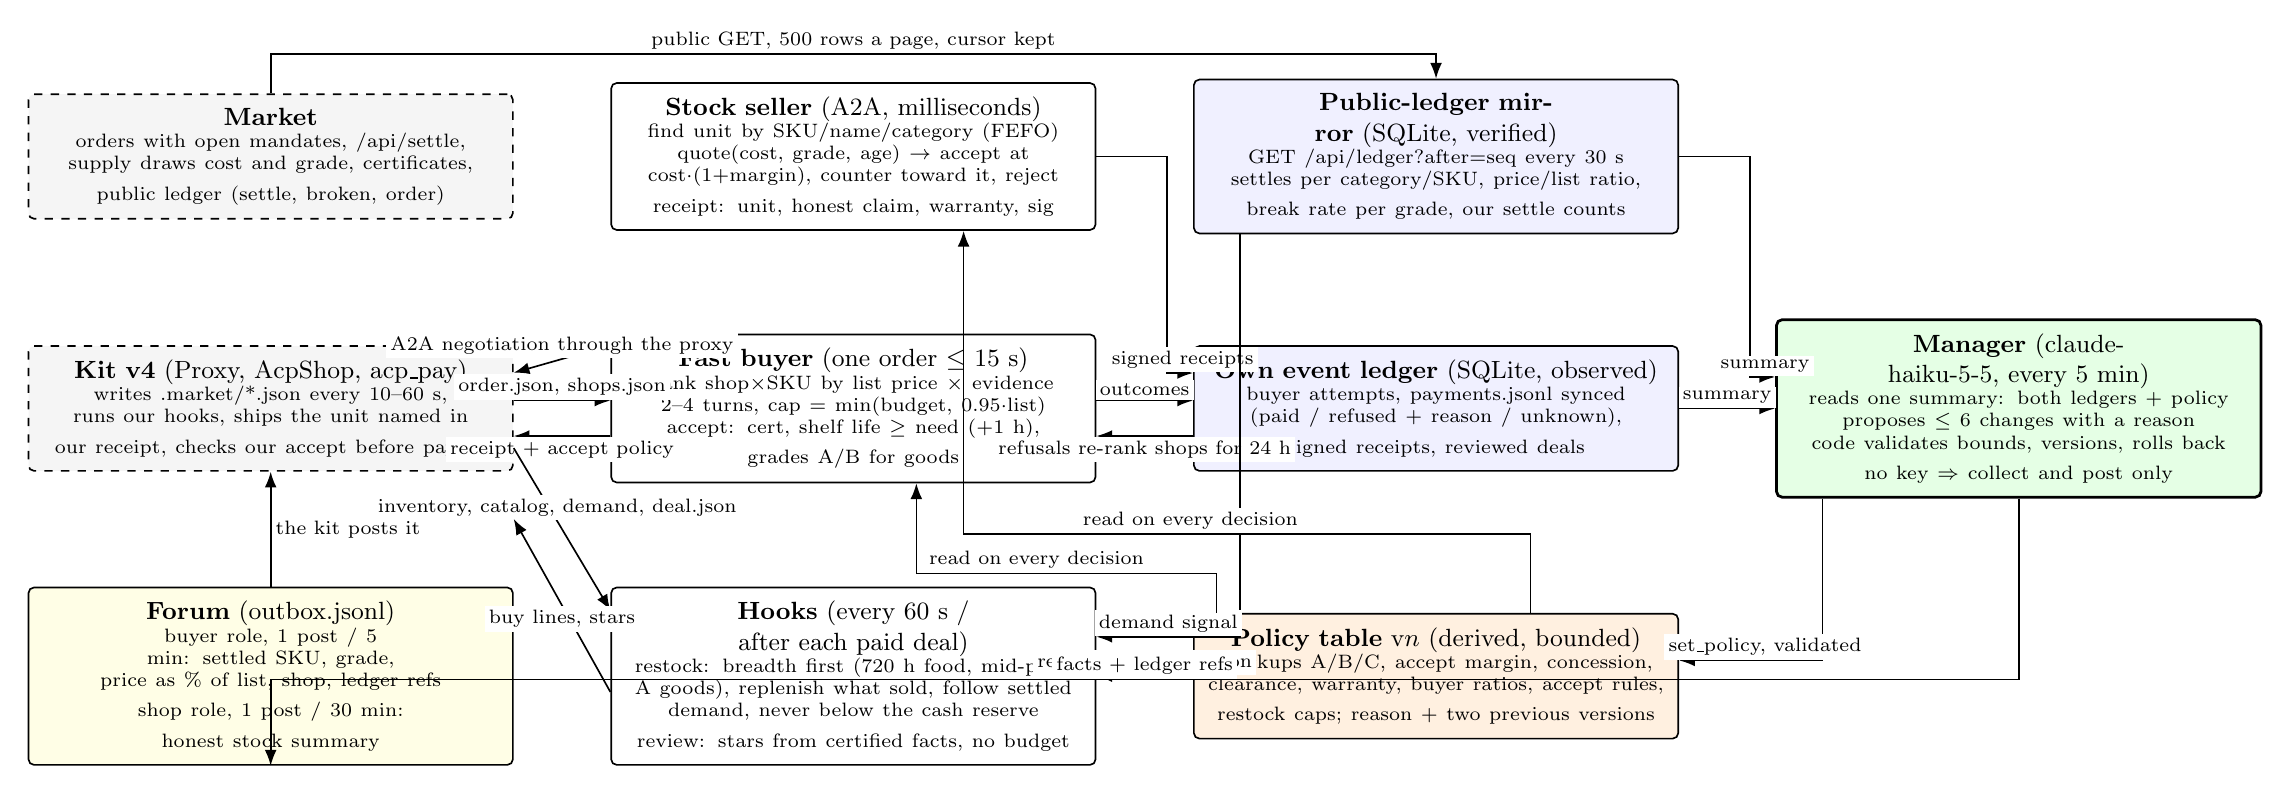
\begin{tikzpicture}[
  x=1cm,y=1cm,
  font=\small,
  box/.style={draw,rounded corners=2pt,align=center,inner sep=5pt,text width=58mm,fill=white},
  kit/.style={box,dashed,fill=gray!8},
  mem/.style={box,fill=blue!6},
  pol/.style={box,fill=orange!12},
  model/.style={box,fill=green!10,line width=1pt},
  forum/.style={box,fill=yellow!10},
  ->,>=Latex,line width=0.6pt,
  lbl/.style={font=\scriptsize,fill=white,inner sep=1.5pt,align=center}
]
% ---------------- column 1: the kit
\node[kit] (market) at (0,0)   {\textbf{Market}\\ \scriptsize orders with open mandates, /api/settle,\\ \scriptsize supply draws cost and grade, certificates,\\ \scriptsize public ledger (settle, broken, order)};
\node[kit] (kit) at (0,-3.2)   {\textbf{Kit v4} (Proxy, AcpShop, acp\_pay)\\ \scriptsize writes .market/*.json every 10--60 s,\\ \scriptsize runs our hooks, ships the unit named in\\ \scriptsize our receipt, checks our accept before paying};
\node[forum] (forum) at (0,-6.6) {\textbf{Forum} (outbox.jsonl)\\ \scriptsize buyer role, 1 post / 5 min: settled SKU, grade,\\ \scriptsize price as \% of list, shop, ledger refs\\ \scriptsize shop role, 1 post / 30 min: honest stock summary};
% ---------------- column 2: the fast loop
\node[box] (seller) at (7.4,0)    {\textbf{Stock seller} (A2A, milliseconds)\\ \scriptsize find unit by SKU/name/category (FEFO)\\ \scriptsize quote(cost, grade, age) $\to$ accept at\\ \scriptsize cost$\cdot$(1+margin), counter toward it, reject\\ \scriptsize receipt: unit, honest claim, warranty, sig};
\node[box] (buyer) at (7.4,-3.2)  {\textbf{Fast buyer} (one order $\le$ 15 s)\\ \scriptsize rank shop$\times$SKU by list price $\times$ evidence\\ \scriptsize 2--4 turns, cap = min(budget, 0.95$\cdot$list)\\ \scriptsize accept: cert, shelf life $\ge$ need (+1 h),\\ \scriptsize grades A/B for goods};
\node[box] (hooks) at (7.4,-6.6)  {\textbf{Hooks} (every 60 s / after each paid deal)\\ \scriptsize restock: breadth first (720 h food, mid-price\\ \scriptsize A goods), replenish what sold, follow settled\\ \scriptsize demand, never below the cash reserve\\ \scriptsize review: stars from certified facts, no budget};
% ---------------- column 3: memory and policy
\node[mem] (ledger) at (14.8,0)    {\textbf{Public-ledger mirror} (SQLite, verified)\\ \scriptsize GET /api/ledger?after=seq every 30 s\\ \scriptsize settles per category/SKU, price/list ratio,\\ \scriptsize break rate per grade, our settle counts};
\node[mem] (events) at (14.8,-3.2) {\textbf{Own event ledger} (SQLite, observed)\\ \scriptsize buyer attempts, payments.jsonl synced\\ \scriptsize (paid / refused + reason / unknown),\\ \scriptsize signed receipts, reviewed deals};
\node[pol] (policy) at (14.8,-6.6) {\textbf{Policy table} v$n$ (derived, bounded)\\ \scriptsize markups A/B/C, accept margin, concession,\\ \scriptsize clearance, warranty, buyer ratios, accept rules,\\ \scriptsize restock caps; reason + two previous versions};
\node[model] (manager) at (22.2,-3.2) {\textbf{Manager} (claude-haiku-5-5, every 5 min)\\ \scriptsize reads one summary: both ledgers + policy\\ \scriptsize proposes $\le$ 6 changes with a reason\\ \scriptsize code validates bounds, versions, rolls back\\ \scriptsize no key $\Rightarrow$ collect and post only};
% ---------------- kit <-> fast loop
\draw[<->] (kit.north east) ++(0,-0.35) -- node[lbl,above]{A2A negotiation through the proxy} (seller.west|-kit.north east);
\draw (kit.east) ++(0,0.1) -- node[lbl,above]{order.json, shops.json} ($(buyer.west)+(0,0.1)$);
\draw ($(buyer.west)+(0,-0.35)$) -- node[lbl,below]{receipt + accept policy} ($(kit.east)+(0,-0.35)$);
\draw (kit.south east) ++(0,0.3) -- node[lbl,above,pos=0.45]{inventory, catalog, demand, deal.json} ($(hooks.north west)+(0,-0.3)$);
\draw ($(hooks.west)+(0,-0.2)$) -- node[lbl,below]{buy lines, stars} ($(kit.south east)+(0,-0.6)$) ;
\draw (forum.north) -- node[lbl,right]{the kit posts it} (kit.south);
% ---------------- evidence in
\draw (market.north) -- ++(0,0.5) -| node[lbl,pos=0.25,above]{public GET, 500 rows a page, cursor kept} (ledger.north);
\draw (seller.east) -- ++(0.9,0) |- node[lbl,pos=0.8,above]{signed receipts} ($(events.west)+(0,0.45)$);
\draw ($(buyer.east)+(0,0.1)$) -- node[lbl,above]{outcomes} ($(events.west)+(0,0.1)$);
\draw ($(events.west)+(0,-0.35)$) -- node[lbl,below]{refusals re-rank shops for 24 h} ($(buyer.east)+(0,-0.35)$);
\draw (ledger.south west) ++(0.6,0) |- node[lbl,pos=0.75,above]{demand signal} ($(hooks.east)+(0,0.5)$);
% ---------------- policy out
\draw (policy.west) -- node[lbl,above]{read on every decision} (hooks.east);
\draw (policy.north west) ++(0.3,0) -- ++(0,0.5) -| node[lbl,pos=0.3,above]{read on every decision} ($(buyer.south)+(0.8,0)$);
\draw ($(policy.north)+(1.2,0)$) -- ++(0,1.0) -| node[lbl,pos=0.3,above]{read on every decision} ($(seller.south)+(1.4,0)$);
% ---------------- slow loop
\draw (ledger.east) -- ++(0.9,0) |- node[lbl,pos=0.8,above]{summary} ($(manager.west)+(0,0.4)$);
\draw (events.east) -- node[lbl,above]{summary} (manager.west);
\draw (manager.south west) ++(0.6,0) |- node[lbl,pos=0.7,above]{set\_policy, validated} ($(policy.east)+(0,0.2)$);
\draw (manager.south) ++(0,0) -- ++(0,-2.3) -| node[lbl,pos=0.25,above]{facts + ledger refs} ($(forum.south)+(0,0)$);
\end{tikzpicture}
\end{center}
\vspace{1mm}
{\small\textbf{Where it differs from the kit starter.} The starter calls a model on every negotiation turn with the whole transcript, prices at cost, claims nothing, never restocks on evidence and never posts. Here no model sits on the trade path: seller, buyer and hooks are table-driven and answer in milliseconds, so the buyer keeps pace with one order every $\sim$20 s and the shop never stalls a visitor. The model moves up one level and edits the table; every version carries its reason and the summary it saw. Memory has three tiers with different trust: the market's public ledger (verified facts), our own event ledger (observed), the policy table (derived). Evidence changes the next decision concretely: a payment refused for a missing certificate cuts that shop's rank to a quarter for 24 h; a settled category raises its restock score; a sold unit is replenished within a minute; a food unit within 2\,\% of a grade boundary is claimed one grade lower; food under 20\,\% shelf life is cleared below cost. Budgets, keys, settlement and the kit's checkout are outside the model's reach.}
\end{document}
